\documentclass[tikz,border=2mm]{standalone}
\usetikzlibrary{decorations.text,arrows.meta,calc}

\usepackage{fontspec}
\setmainfont{Fira Sans}

\tikzset{curved text/.style={decorate,
        decoration={text effects along path,
            text={#1}, text align=center,
            text effects/.cd, text along path}}}

\begin{document}
    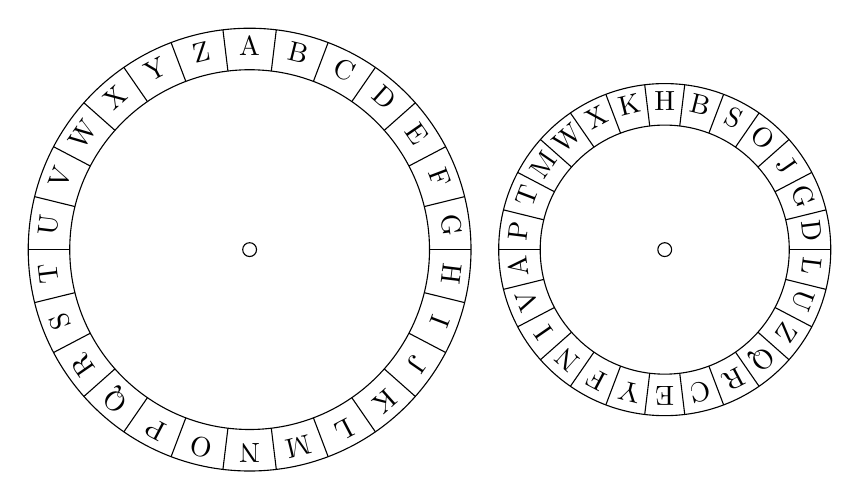
\begin{tikzpicture}[x=1em,y=1em]
    \draw (0,0) circle [radius=0.25,black];
    \draw (15,0) circle [radius=0.25,black];

    \pgfmathsetmacro\angdiv{360/26}
    \coordinate (n-0) at (90+\angdiv/2:7) {};
    \coordinate (m-0) at (14.4,5) +(90-\angdiv/2:5) {};

    \draw circle [radius=8] circle [radius=6.5];
    \draw (15,0) circle [radius=6] circle [radius=4.5];
    \foreach \i in {0,...,25}{
        \draw ($({90-(\i-1/2)*\angdiv}:8)$) -- ($(({90-(\i-1/2)*\angdiv}:6.5)$);
        \draw ($(15,0) +({90-(\i-1/2)*\angdiv}:4.5)$) -- ($(15,0) +(({90-(\i-1/2)*\angdiv}:6)$);
    };

    \foreach [count=\a from 0] \text in {A,...,Z}{
        \pgfmathtruncatemacro\b{\a+1}%
        \path [curved text=\text] (n-\a) arc [start angle=90-(\a-1/2)*\angdiv, delta angle=-\angdiv, radius=7] node (n-\b) {};
    }
    \foreach [count=\a from 0] \text in {H,B,S,O,J,G,D,L,U,Z,Q,R,C,E,Y,F,N,I,V,A,P,T,M,W,X,K}{
        \pgfmathtruncatemacro\b{\a+1}%
        \path [curved text=\text] (m-\a) arc [start angle=90-(\a-1/2)*\angdiv, delta angle=-\angdiv, radius=5] node (m-\b) {}; % Inner circle
    }
    \end{tikzpicture}
\end{document}
